
\documentclass[a4paper,10pt]{article}
\usepackage[top=2cm, left=2.5cm, right=2.5cm, bottom=2cm]{geometry}
\usepackage[cmex10]{amsmath}
\usepackage{graphicx}
\usepackage{gvv-book}
\usepackage{gvv}
\usepackage{textcomp}
\usepackage{multicol}

\begin{document}

\title{2017 - AR : Architecture and Planning Exam}
\author{Puni Aditya - EE25BTECH11046}
\date{13th August, 2025}
\maketitle
Duration: Three Hours \hfill Maximum Marks:100

\section*{Q.1 - Q.25 carry one mark each.}

\begin{enumerate}
    \item The Pritzker Architecture prize for the year 2016 has been awarded to 
    \begin{multicols}{2}
	\begin{enumerate}
        \item Alejandro Aravena
        \item Frei Otto
        \item Stephen Breyer
        \item Yung Ho Chang
    \end{enumerate}
	\end{multicols}
    \hfill (GATE-AR 2017)
    
    \item As per the CPWD Handbook on Barrier Free and Accessibility, 2014, Government of India, the minimum length of a straight ramp in metre to raise a wheelchair to the plinth level of 600 mm, is \rule{2cm}{0.4pt}
    \hfill (GATE-AR 2017)
    
    \item Tuscan and Composite orders are associated with 
    \begin{multicols}{2}
	\begin{enumerate}
        \item Greek Architecture
        \item Islamic Architecture
        \item Byzantine Architecture
        \item Roman Architecture
    \end{enumerate}
	\end{multicols}
    \hfill (GATE-AR 2017)
    
    \item A pointed arch having two centres and radii greater than the span is known as 
    \begin{multicols}{2}
	\begin{enumerate}
        \item Lancet arch
        \item Gothic arch
        \item Roman arch
        \item Drop arch
    \end{enumerate}
	\end{multicols}
    \hfill (GATE-AR 2017)

    \item The concepts of 'serial vision', 'punctuation' and 'closure' were proposed by 
    \begin{multicols}{2}
	\begin{enumerate}
        \item Le Corbusier
        \item Louis Kahn
        \item Gordon Cullen
        \item Kevin Lynch
    \end{enumerate}
	\end{multicols}
    \hfill (GATE-AR 2017)
    
    \item In one litre of paint, volume of solid pigment and volume of non-volatile binder are 400 cc and 600 cc respectively. The Pigment Volume Concentration number of the paint is \rule{2cm}{0.4pt}
    \hfill (GATE-AR 2017)
    
    \item 'Cold joint' refers to the 
    \begin{enumerate}
        \item expansion joint in large span concrete members
        \item interface between an already setting concrete and a fresh batch of concrete
        \item structural crack arrested by embedding metal rods
        \item joining of two similar metals in vacuum
    \end{enumerate}
    \hfill (GATE-AR 2017)

    \item Slenderness ratio of a column is represented as: 
    \begin{multicols}{2}
    \begin{enumerate}
        \item Effective length/Cross-sectional area
        \item Effective length/Radius of gyration
        \item Actual length/Cross-sectional area
        \item Actual length/Radius of gyration
    \end{enumerate}
    \end{multicols}
    \hfill (GATE-AR 2017)

	\item Liquidated damage refers to the 
    \begin{enumerate}
        \item cost borne by the contractor to rectify defects within defect-liability period
        \item compensation paid on breach of contract to the affected party by the other party
        \item money paid by the insurance company to the owner of insured property if it is damaged
        \item money earned by the owner from selling damaged property through auction
    \end{enumerate}
    \hfill (GATE-AR 2017)
    
    \item Which of the following processes is \textbf{NOT} used for corrosion resistance of cast iron? 
    \begin{multicols}{4}
	\begin{enumerate}
        \item Painting
        \item Epoxy coating
        \item Quenching
        \item Galvanizing
    \end{enumerate}
	\end{multicols}
    \hfill (GATE-AR 2017)
    
    \item Data on 'households with one or more married couples sharing room with a person aged 12 years or more', is used for computing 
    \begin{multicols}{2}
	\begin{enumerate}
        \item housing density
        \item housing shortage
        \item housing price
        \item housing affordability
    \end{enumerate}
	\end{multicols}
    \hfill (GATE-AR 2017)
    
    \item Excellence in Design for Greater Efficiency (EDGE) programme \textbf{DOES NOT} focus on 
    \begin{multicols}{2}
	\begin{enumerate}
        \item lower carbon emission
        \item greater resource efficiency
        \item cost effectiveness
        \item labour safety
    \end{enumerate}
	\end{multicols}
    \hfill (GATE-AR 2017)
    
    \item Select the right option representing strategic components arranged in ascending order of specified minimum area under Smart City Mission of Government of India. 
    \begin{enumerate}
        \item Greenfield development - Redevelopment - Retrofitting
        \item Redevelopment - Greenfield development - Retrofitting
        \item Retrofitting - Redevelopment - Greenfield development
        \item Redevelopment - Retrofitting - Greenfield development
    \end{enumerate}
    \hfill (GATE-AR 2017)
    
    \item The grade-separated interchange suitable for 3-legged road intersection is: 
    \begin{multicols}{4}
	\begin{enumerate}
        \item Trumpet
        \item Full Clover leaf
        \item Diamond
        \item Partial Clover leaf
    \end{enumerate}
	\end{multicols}
    \hfill (GATE-AR 2017)
    
    \item The design element provided to ensure safety of a vehicle travelling at a prescribed design speed along the curved segment of a highway is 
    \begin{multicols}{4}
	\begin{enumerate}
        \item shoulder
        \item super-elevation
        \item median
        \item footpath
    \end{enumerate}
	\end{multicols}
    \hfill (GATE-AR 2017)
    
    \item Which of the following processes is \textbf{NOT} adopted in solid waste management? 
    \begin{multicols}{4}
	\begin{enumerate}
        \item Incineration
        \item Pyrolysis
        \item Flocculation
        \item Sanitary landfill
    \end{enumerate}
	\end{multicols}
    \hfill (GATE-AR 2017)
    
    \item The principle of Eminent Domain is the power to 
    \begin{enumerate}
        \item restrict exercise of rights in land through zoning and environmental laws
        \item control land use
        \item retain land use
        \item acquire and take possession of property in order to promote public interest
    \end{enumerate}
    \hfill (GATE-AR 2017)
    
    \item In which of the following models does the private partner own the revenue as well as the risk associated with the project for a limited period of time? 
    \begin{enumerate}
        \item Build, Own, Operate (BOO)
        \item Build, Own, Operate, Transfer (BOOT)
        \item Design, Build, Finance, Operate (DBFO)
        \item Design, Bid, Build (DBB)
    \end{enumerate}
    \hfill (GATE-AR 2017)

	\item In a multi-storied building, the type of plumbing system suitable for reusing the sullage for non-potable use is 
    \begin{multicols}{2}
	\begin{enumerate}
        \item single stack system
        \item partially ventilated single stack system
        \item one pipe system
        \item two pipe system
    \end{enumerate}
	\end{multicols}
    \hfill (GATE-AR 2017)

	\item The unit for measuring sound absorption in a room is 
    \begin{multicols}{4}
	\begin{enumerate}
        \item Sabin
        \item Phon
        \item Decibel
        \item Hertz
    \end{enumerate}
	\end{multicols}
    \hfill (GATE-AR 2017)

    \item In Geographic Information System, DEM represents information on 
    \begin{multicols}{4}
	\begin{enumerate}
        \item vegetation cover
        \item soil type
        \item water table
        \item topography
    \end{enumerate}
	\end{multicols}
    \hfill (GATE-AR 2017)

    \item Minimum points required for GRIHA certification is 
    \begin{multicols}{4}
	\begin{enumerate}
        \item 35
        \item 40
        \item 50
        \item 60
    \end{enumerate}
	\end{multicols}
    \hfill (GATE-AR 2017)

    \item ArchiCAD, Auto Desk Revit, Digital Project Designer (CATIA) and Vector Works Architect are examples of 
    \begin{multicols}{2}
	\begin{enumerate}
        \item Statistical Analysis software
        \item GIS software
        \item BIM software
        \item Image processing software
    \end{enumerate}
	\end{multicols}
    \hfill (GATE-AR 2017)

    \item The CARTOSAT 2C satellite recently launched by ISRO 
    \begin{multicols}{2}
    \begin{enumerate}
        \item is a geo-synchronous satellite
        \item is a part of IRNSS GPS satellite system
        \item was launched using a GSLV rocket
        \item has high spatial resolution
    \end{enumerate}
    \end{multicols}
    \hfill (GATE-AR 2017)

    \item Which of the following trees has a columnar form? 
    \begin{multicols}{2}
	\begin{enumerate}
        \item Delonix regia
        \item Tamarindus indica
        \item Polyalthia longifolia
        \item Callistemon lanceolatus
    \end{enumerate}
	\end{multicols}
    \hfill (GATE-AR 2017)

\section*{Q.26 to Q.55 carry two marks each.}

    \item Match the architectural movements in \textbf{Group-I} with their proponents in \textbf{Group-II}. \\
    \begin{tabular}{ l l }
	\textbf{Group-I} & \textbf{Group-II} \\
	P. Deconstruction & 1. Joseph Paxton \\
	Q. Historicism & 2. Kenzo Tange \\
	R. Metabolism & 3. Walter Gropius \\
	S. Art Nouveau & 4. Victor Horta \\
	& 5. Frank O. Gehry \\
	\end{tabular}
	\begin{multicols}{2}
	\begin{enumerate}
        \item P-5, Q-1, R-2, S-4
        \item P-5, Q-4, R-2, S-3
        \item P-5, Q-2, R-3, S-3
        \item P-2, Q-4, R-1, S-5
    \end{enumerate}
	\end{multicols}
    \hfill (GATE-AR 2017)
    
    \item Associate the historic buildings in \textbf{Group-I} with their predominant materials in \textbf{Group-II}. \\
    \begin{tabular}{ l l }
	\textbf{Group-I} & \textbf{Group-II} \\
	P. Lingaraj Temple, Bhubaneshwar, India & 1. Red sandstone \\
	Q. Victoria Memorial, Kolkata, India & 2. Timber \\
	R. Padmanabhapuram Palace, Thuckalay, India & 3. Terracotta tiles \\
	S. Humayun's Tomb, Delhi, India & 4. Sandstone and laterite \\
	& 5. Marble \\
	\end{tabular}
	\begin{multicols}{2}
	\begin{enumerate}
        \item P-1, Q-2, R-3, S-5
        \item P-1, Q-4, R-3, S-5
        \item P-2, Q-1, R-3, S-4
        \item P-4, Q-5, R-2, S-1
    \end{enumerate}
	\end{multicols}
    \hfill (GATE-AR 2017)
    
    \item Match the terminologies in \textbf{Group-I} with their description in \textbf{Group-II}. \\
    \begin{tabular}{ l l }
	\textbf{Group-I} & \textbf{Group-II} \\
	P. Pruning & 1. Cutting of trees \\
	Q. Felling & 2. Removing broken branches from trees for better growth \\
	R. Hoeing & 3. Maintaining moisture content in soil by a protective layer \\
	S. Mulching & 4. Indiscriminate cutting of branches to reduce the size of a tree \\
	& 5. Loosening the ground to remove weeds \\
	\end{tabular}
	\begin{multicols}{2}
	\begin{enumerate}
        \item P-2, Q-1, R-5, S-3
        \item P-2, Q-1, R-4, S-3
        \item P-2, Q-1, R-3, S-4
        \item P-1, Q-2, R-3, S-1
    \end{enumerate}
	\end{multicols}
    \hfill (GATE-AR 2017)

	\item A proposed housing will have HIG, MIG and LIG units on a site measuring 60,750 sq.m. The buildable area of each category of units with respect to the total buildable area will be 30\%, 50\% and 20\% respectively. The maximum allowable FAR is 2.5, ground coverage 45\% and height 15 m. The maximum buildable area in sq.m of HIG units, considering a floor height of 3 m for all categories will be \rule{2cm}{0.4pt}
    \hfill (GATE-AR 2017)
    
    \item In 2011, the population of a town was 5,00,000 and the number of housing units were 1,00,000. Calculate the additional number of dwelling units (DU) required by 2031 so that there is no housing shortage. The assumptions are
    \begin{itemize}
    \item 5\% decadal increase in population
    \item New DU to be completed by 2021 is 10,000
    \item Number of DU which will become non habitable by 2031 is 5,000
    \item Average household size is 4.5 
    \end{itemize}
    \hfill (GATE-AR 2017)
    
    \item Match the classical urban planning theories in \textbf{Group-I} with their proponents in \textbf{Group-II}. \\
    \begin{tabular}{ l l }
	\textbf{Group-I} & \textbf{Group-II} \\
	P. Concentric Zone Model & 1. Berry and Horton \\
	Q. Sector Model & 2. Homer Hoyt \\
	R. Multiple Nuclei Model & 3. Ernest Burgess \\
	S. Factorial Ecology & 4. Shevky and Bell \\
	& 5. Harris and Ullman \\
	\end{tabular}
	\begin{multicols}{2}
	\begin{enumerate}
        \item P-4, Q-1, R-3, S-5
        \item P-3, Q-2, R-3, S-5
        \item P-2, Q-4, R-5, S-1
        \item P-3, Q-2, R-5, S-1
    \end{enumerate}
	\end{multicols}
    \hfill (GATE-AR 2017)

    \item Match the distinguished housing projects in \textbf{Group-I} with their architects in \textbf{Group-II}. \\
    \begin{tabular}{ l l }
	\textbf{Group-I} & \textbf{Group-II} \\
	P. Nagakin Capsule Tower, Tokyo, Japan & 1. Walter Gropius \\
	Q. Tara Apartment, New Delhi, India & 2. Moshe Safdie \\
	R. Habitat 67, Montreal, Canada & 3. Ralph Erskine \\
	S. Byker Wall, New Castle, England & 4. Charles Correa \\
	& 5. Kisho Kurokawa \\
	\end{tabular}
	\begin{multicols}{2}
	\begin{enumerate}
        \item P-5, Q-4, R-2, S-3
        \item P-1, Q-3, R-4, S-5
        \item P-5, Q-2, R-1, S-4
        \item P-5, Q-4, R-2, S-1
    \end{enumerate}
	\end{multicols}
    \hfill (GATE-AR 2017)

    \item Match the development schemes by Government of India in \textbf{Group-I} with their objectives in \textbf{Group-II}. \\
    \begin{tabular}{ l l }
	\textbf{Group-I} & \textbf{Group-II} \\
	P. PMAY & 1. Housing for All \\
	Q. AMRUT & 2. Rural cluster development \\
	R. NRUM & 3. Heritage city development \\
	S. HRIDAY & 4. Urban mobility improvement \\
	& 5. Urban rejuvenation \\
	\end{tabular}
	\begin{multicols}{2}
	\begin{enumerate}
        \item P-1, Q-5, R-4, S-3
        \item P-1, Q-5, R-2, S-3
        \item P-3, Q-5, R-1, S-2
        \item P-4, Q-2, R-1, S-5
    \end{enumerate}
	\end{multicols}
    \hfill (GATE-AR 2017)

    \item Match the international events in \textbf{Group-I} with their directives in \textbf{Group-II}. \\
    \begin{tabular}{ l l }
	\textbf{Group-I} & \textbf{Group-II} \\
	P. Earth Summit, Rio de Janeiro, 1992 & 1. Kyoto Protocol \\
	Q. UN Framework Convention on Climate Change, New York, 1992 & 2. Agenda 21 \\
	R. UN Sustainable Development Summit, New York, 2015 & 3. Heritage conservation \\
	S. Habitat II, Istanbul, 1996 & 4. Agenda 2030 \\
	& 5. Housing for All \\
	\end{tabular}
	\begin{multicols}{2}
	\begin{enumerate}
        \item P-1, Q-5, R-4, S-3
        \item P-1, Q-5, R-2, S-3
        \item P-2, Q-1, R-4, S-5
        \item P-2, Q-1, R-5, S-4
    \end{enumerate}
	\end{multicols}
    \hfill (GATE-AR 2017)

    \item Match the planning techniques in \textbf{Group-I} with their salient features in \textbf{Group-II}. \\
    \begin{tabular}{ l l }
	\textbf{Group-I} & \textbf{Group-II} \\
	P. Land pooling & 1. Assigning specific task on a short time horizon \\
	Q. Action Plan & 2. Assembling privately owned land parcels for development \\
	R. Land sharing & 3. Agreement for reallocation of land between occupiers and owners \\
	S. Transfer of Development Rights & 4. Assigning specific task on a long time horizon \\
	& 5. Incentive based voluntary shifting of FAR of a plot to another plot \\
	\end{tabular}
	\begin{multicols}{2}
	\begin{enumerate}
        \item P-1, Q-5, R-4, S-3
        \item P-2, Q-1, R-3, S-5
        \item P-2, Q-1, R-3, S-4
        \item P-4, Q-2, R-1, S-5
    \end{enumerate}
	\end{multicols}
    \hfill (GATE-AR 2017)

    \item For a symmetrical two dimensional truss as shown in the figure, vertical force in kN acting on the member PQ is \rule{2cm}{0.4pt}
    \begin{figure}[h!]
        \centering
        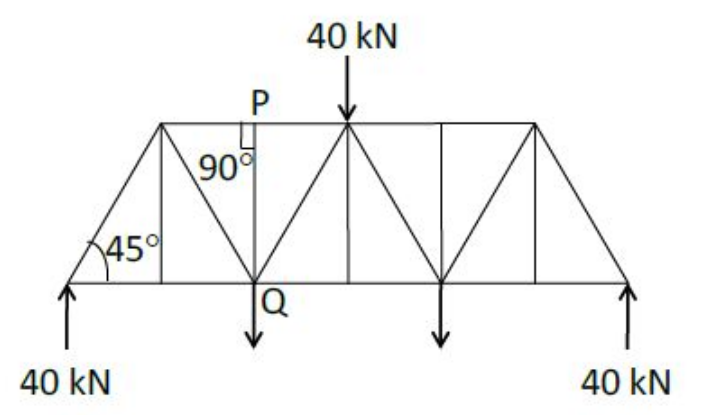
\includegraphics[width=0.5\columnwidth]{figs/01.jpg}
        \caption{Symmetrical Truss with 40 kN loads}
	\label{fig:Img01}
	\end{figure}
    \hfill (GATE-AR 2017)

    \item Value of bending moment in kN-m at point C for a beam as shown in the figure is \rule{2cm}{0.4pt}
    \begin{figure}[h!]
        \centering
        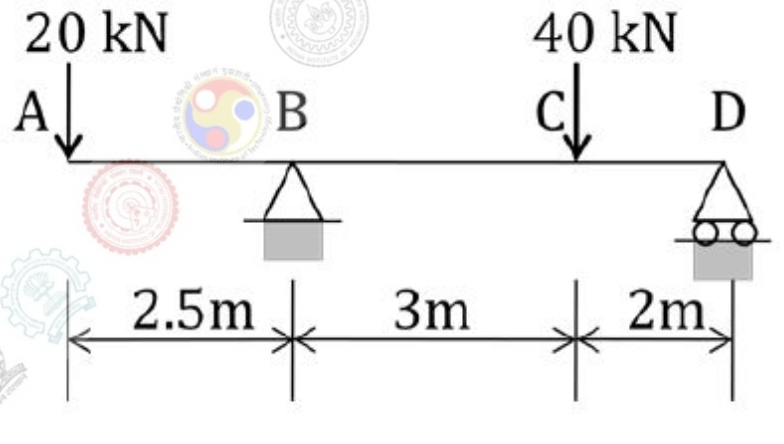
\includegraphics[width=0.5\columnwidth]{figs/02.jpg}
        \caption{Beam with loads}
	\label{fig:Img02}
	\end{figure}
    \hfill (GATE-AR 2017)

    \item Fee of contractor for a project has the following provisions
    \begin{itemize}
    \item Basic fee: 15\% of actual cost of work incurred
    \item Bonus: 20\% of savings from estimated cost of work
    \item Penalty: 20\% of cost overrun
    \end{itemize}
    If the estimated cost of the project is Rs. 60,000, and the actual cost is Rs. 70,000, then the total fee of contractor in Rupees is \rule{2cm}{0.4pt}
    \hfill (GATE-AR 2017)

    \item A site has a unidirectional slope of 30\textdegree with horizontal along its longer side. The projected dimensions of the site on the horizontal plane measures 30 m $\times$ 40 m. Using cut and fill method the site has to be levelled parallel to the horizontal plane. The minimum amount of earth to be excavated in cubic metre is \rule{2cm}{0.4pt}
    \hfill (GATE-AR 2017)

    \item The optimistic, most-likely and pessimistic time for developing a new product are 12 months, 15 months and 17 months, respectively. Calculate the expected time in months. 
    \hfill (GATE-AR 2017)

    \item A circular plate inclined at an angle $\theta$ with horizontal plane generates an ellipse as top view with major axis and minor axis of 5 cm and 2.5 cm respectively. The value of $\theta$ in degrees is \rule{2cm}{0.4pt}
    \hfill (GATE-AR 2017)

    \item Calculate the volume of cement in cubic metre required for making 10 cubic metre of M20 grade Plain Cement Concrete work, assuming the ratio of dry concrete mix to wet concrete mix as 1.52. 
    \hfill (GATE-AR 2017)

    \item One acre of agricultural land has been given on a lease till perpetuity at an annual rent of Rs. 10,000 to be paid at the end of each year. Net Present Value of the land parcel in Rupees assuming a discount rate of 5\% per annum is \rule{2cm}{0.4pt}
    \hfill (GATE-AR 2017)

    \item In year 2001, a district with 4,000 manufacturing jobs had a 10\% share of total manufacturing jobs within the state. In year 2011, the state recorded 15\% drop in manufacturing jobs whereas, share of the district in total manufacturing jobs within the state increased to 15\%. Additional manufacturing jobs created in the district between year 2001 and 2011 is \rule{2cm}{0.4pt}
    \hfill (GATE-AR 2017)

    \item Match the parameters in \textbf{Group-I} with their units in \textbf{Group-II} \\
    \begin{tabular}{ l l }
	\textbf{Group-I} & \textbf{Group-II} \\
	P. Traffic flow & 1. Metre \\
	Q. Traffic density & 2. Cycles/second \\
	R. Right of Way & 3. Seconds \\
	S. Traffic signal cycle length & 4. Vehicle/km \\
	& 5. PCU/hr \\
	\end{tabular}
	\begin{multicols}{2}
	\begin{enumerate}
        \item P-5, Q-4, R-1, S-2
        \item P-5, Q-4, R-1, S-3
        \item P-5, Q-2, R-4, S-3
        \item P-4, Q-5, R-1, S-3
    \end{enumerate}
	\end{multicols}
    \hfill (GATE-AR 2017)

    \item Match the planning tasks in \textbf{Group-I} with the tools of analysis in \textbf{Group-II} \\
    \begin{tabular}{ l l }
	\textbf{Group-I} & \textbf{Group-II} \\
	P. Population projection & 1. Input-Output Analysis \\
	Q. Regional resource allocation & 2. Hardy Cross Method \\
	R. Trip distribution & 3. Cohort Analysis \\
	S. Design of water distribution network & 4. Gravity Model \\
	& 5. Moving observer method \\
	\end{tabular}
	\begin{multicols}{2}
	\begin{enumerate}
        \item P-3, Q-1, R-4, S-2
        \item P-3, Q-5, R-4, S-1
        \item P-5, Q-1, R-3, S-4
        \item P-1, Q-3, R-5, S-2
    \end{enumerate}
	\end{multicols}
    \hfill (GATE-AR 2017)

    \item Match the land use classes in \textbf{Group-I} with the use zones in \textbf{Group-II} \\
    \begin{tabular}{ l l }
	\textbf{Group-I} & \textbf{Group-II} \\
	P. Transportation & 1. Sports complex \\
	Q. Commercial & 2. Heritage and conservation areas \\
	R. Public and Semi-public & 3. Burial ground \\
	S. Recreational & 4. BRT corridor \\
	& 5. Service sector \\
	\end{tabular}
	\begin{multicols}{2}
	\begin{enumerate}
        \item P-4, Q-1, R-3, S-5
        \item P-5, Q-3, R-1, S-2
        \item P-4, Q-5, R-1, S-2
        \item P-4, Q-5, R-3, S-1
    \end{enumerate}
	\end{multicols}
    \hfill (GATE-AR 2017)

    \item Associate the structural systems in \textbf{Group-I} with the buildings in \textbf{Group-II}. \\
    \begin{tabular}{ l l }
	\textbf{Group-I} & \textbf{Group-II} \\
	P. Folded plates & 1. Kurilpa Bridge, Brisbane \\
	Q. Shell & 2. Eden Project, Cornwall \\
	R. Tensegrity & 3. Riverside Museum, Glasgow \\
	S. Pneumatic & 4. MIT Auditorium, Boston \\
	& 5. 30, St. Mary Axe, London \\
	\end{tabular}
	\begin{multicols}{2}
	\begin{enumerate}
        \item P-3, Q-4, R-1, S-2
        \item P-5, Q-4, R-3, S-1
        \item P-3, Q-2, R-1, S-5
        \item P-1, Q-3, R-4, S-2
    \end{enumerate}
	\end{multicols}
    \hfill (GATE-AR 2017)

    \item As per National Building Code of India, 2005, the maximum number of occupants per unit exit width of a doorway is 60, where unit exit width is 500 mm. The maximum permissible occupants in a theatre having four number of 2.2 m wide doors will be \rule{2cm}{0.4pt}
    \hfill (GATE-AR 2017)

    \item Match the instruments in \textbf{Group-I} with the corresponding tests in \textbf{Group-II}. \\
    \begin{tabular}{ l l }
	\textbf{Group-I} & \textbf{Group-II} \\
	P. Pycnometer & 1. Initial and final setting time \\
	Q. Brinell's Apparatus & 2. Abrasion test \\
	R. Los Angeles Apparatus & 3. Surface hardness test \\
	S. Vicat's Apparatus & 4. Slump test \\
	& 5. Apparent Specific gravity \\
	\end{tabular}
	\begin{multicols}{2}
	\begin{enumerate}
        \item P-5, Q-3, R-2, S-1
        \item P-5, Q-4, R-2, S-1
        \item P-3, Q-2, R-1, S-5
        \item P-2, Q-3, R-4, S-1
    \end{enumerate}
	\end{multicols}
    \hfill (GATE-AR 2017)

    \item Water flows through a constricted circular pipe whose diameter at the constricted end is half of the non-constricted end. Velocity of water at the non-constricted end is 2 m/s. Velocity of water in m/s at the constricted end using the principle of continuity of flow is \rule{2cm}{0.4pt}
    \hfill (GATE-AR 2017)

    \item A drainage basin of 180 hectares comprises 40\% wooded area, 45\% grassed area and 15\% paved area. Runoff coefficients for wooded, grassed and paved areas are 0.01, 0.2 and 0.95 respectively. The composite runoff coefficient for the drainage basin is \rule{2cm}{0.4pt}
    \hfill (GATE-AR 2017)

    \item A fluorescent light source consumes 40 W electric power and has a luminous efficacy of 40 lm/W. Illumination in lux at a distance of 3 m from this light source is \rule{2cm}{0.4pt}
    \hfill (GATE-AR 2017)

    \item A room measures 3 m (width) $\times$ 4 m (length) $\times$ 3 m (height). The outdoor temperature is 36\textdegree C. The volumetric specific heat of air is 1300 J/cu.m.\textdegree C. The ventilation heat flow rate in Watts required to attain an internal room temperature of 26\textdegree C with 3 air changes per hour is \rule{2cm}{0.4pt}
    \hfill (GATE-AR 2017)

    \item Match the equipment in \textbf{Group-I} with their applications in \textbf{Group-II}. \\
    \begin{tabular}{ l l }
	\textbf{Group-I} & \textbf{Group-II} \\
	P. PIR & 1. Air conditioning \\
	Q. FCU & 2. Lighting \\
	R. OLED & 3. Power generation \\
	S. BIPV & 4. Motion detection \\
	& 5. Daylight sensing \\
	\end{tabular}
	\begin{multicols}{2}
	\begin{enumerate}
        \item P-4, Q-5, R-2, S-1
        \item P-1, Q-4, R-5, S-3
        \item P-4, Q-1, R-2, S-3
        \item P-4, Q-2, R-5, S-1
    \end{enumerate}
	\end{multicols}
    \hfill (GATE-AR 2017)

\section*{General Aptitude (Q.56 to Q.65)}

    \item He was one of my best \rule{2cm}{0.4pt} and I felt his loss \rule{2cm}{0.4pt}.
    \begin{multicols}{4}
	\begin{enumerate}
        \item friend, keenly
        \item friends, keen
        \item friend, keener
        \item friends, keenly
    \end{enumerate}
	\end{multicols}
    \hfill (GATE-AR 2017)

    \item As the two speakers became increasingly agitated, the debate became \rule{2cm}{0.4pt}.
    \begin{multicols}{4}
	\begin{enumerate}
        \item lukewarm
        \item poetic
        \item forgiving
        \item heated
    \end{enumerate}
	\end{multicols}
    \hfill (GATE-AR 2017)

    \item A right-angled cone (with base radius 5 cm and height 12 cm), as shown in the figure below, is rolled on the ground keeping the point P fixed until the point Q (at the base of the cone, as shown) touches the ground again. \\
    \begin{figure}[h!]
        \centering
        
\includegraphics[width=0.5\columnwidth]{figs/03.jpg}
        \caption{Right-Angled Cone}
	\label{fig:Img03}
	\end{figure}
    By what angle (in radians) about P does the cone travel?
    \begin{multicols}{2}
	\begin{enumerate}
        \item $\frac{5\pi}{12}$
        \item $\frac{5\pi}{24}$
        \item $\frac{24\pi}{5}$
        \item $\frac{10\pi}{13}$
    \end{enumerate}
	\end{multicols}
    \hfill (GATE-AR 2017)

    \item In a company with 100 employees, 45 earn Rs. 20,000 per month, 25 earn Rs. 30,000, 20 earn Rs. 40,000, 8 earn Rs. 60,000, and 2 earn Rs. 150,000. The median of the salaries is 
    \begin{multicols}{4}
	\begin{enumerate}
        \item Rs. 20,000
        \item Rs. 30,000
        \item Rs. 32,300
        \item Rs. 40,000
    \end{enumerate}
	\end{multicols}
    \hfill (GATE-AR 2017)

    \item P, Q, and R talk about S's car collection. P states that S has at least 3 cars. Q believes that S has less than 3 cars. R indicates that to his knowledge, S has at least one car. Only one of P, Q and R is right. The number of cars owned by S is 
    \begin{multicols}{4}
	\begin{enumerate}
        \item 0
        \item 1
        \item 3
        \item Cannot be determined
    \end{enumerate}
	\end{multicols}
    \hfill (GATE-AR 2017)

    \item "Here, throughout the early 1820s, Stuart continued to fight his losing battle to allow his sepoys to wear their caste-marks and their own choice of facial hair on parade, being again reprimanded by the commander-in-chief. His retort that 'A stronger instance than this of European prejudice with relation to this country has never come under my observations' had no effect on his superiors." \\
    According to this paragraph, which of the statements below is most accurate?
    \begin{enumerate}
        \item Stuart's commander-in-chief was moved by this demonstration of his prejudice.
        \item The Europeans were accommodating of the sepoys' desire to wear their caste-marks.
        \item Stuart's 'losing battle' refers to his inability to succeed in enabling sepoys to wear caste-marks.
        \item The commander-in-chief was exempt from the European prejudice that dictated how the sepoys were to dress.
    \end{enumerate}
    \hfill (GATE-AR 2017)

    \item What is the sum of the missing digits in the subtraction problem below? \\
    \begin{figure}[h!]
        \centering
        
\includegraphics[width=0.3\columnwidth]{figs/04.jpg}
        \caption{Problem}
	\label{fig:Img04}
	\end{figure}
    \begin{multicols}{4}
	\begin{enumerate}
        \item 8
        \item 10
        \item 11
        \item Cannot be determined
    \end{enumerate}
	\end{multicols}
    \hfill (GATE-AR 2017)

    \item Let $S_1$ be the plane figure consisting of the points $(x, y)$ given by the inequalities $|x - 1| \leq 2$ and $|y + 2| \leq 3$. Let $S_2$ be the plane figure given by the inequalities $x - y \geq -2$, $y \geq 1$ and $x \leq 3$. Let $S$ be the union of $S_1$ and $S_2$. The area of $S$ is 
    \begin{multicols}{4}
	\begin{enumerate}
        \item 26
        \item 28
        \item 32
        \item 34
    \end{enumerate}
	\end{multicols}
    \hfill (GATE-AR 2017)

    \item Two very famous sportsmen Mark and Steve happened to be brothers, and played for country K. Mark teased James, an opponent from country E. "There is no way you are good enough to play for your country." James replied, "Maybe not, but at least I am the best player in my own family." \\
    Which one of the following can be inferred from this conversation?
    \begin{enumerate}
        \item Mark was known to play better than James
        \item Steve was known to play better than Mark
        \item James and Steve were good friends
        \item James played better than Steve
    \end{enumerate}
    \hfill (GATE-AR 2017)

    \item The growth of bacteria (lactobacillus) in milk leads to curd formation. A minimum bacterial population density of 0.8 (in suitable units) is needed to form curd. In the graph below, the population density of lactobacillus in 1 litre of milk is plotted as a function of time, at two different temperatures, 25\textdegree C and 37\textdegree C. \\
    \begin{figure}[h!]
        \centering
        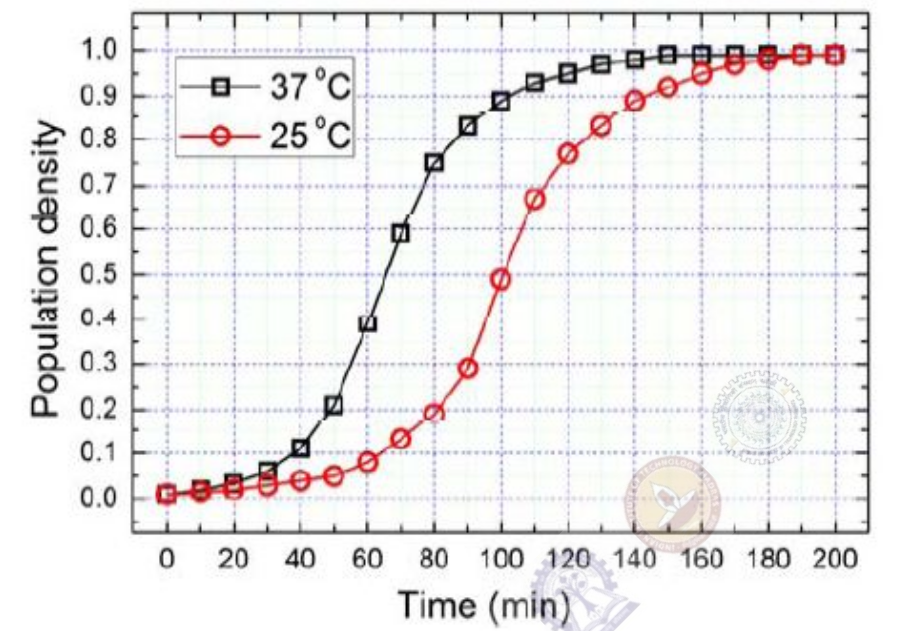
\includegraphics[width=0.5\columnwidth]{figs/05.jpg}
        \caption{Bacterial population density vs Time}
	\label{fig:Img05}
	\end{figure}
    Consider the following statements based on the data shown above: \\
    \begin{itemize}
    \item The growth in bacterial population stops earlier at 37\textdegree C as compared to 25\textdegree C
    \item The time taken for curd formation at 25\textdegree C is twice the time taken at 37\textdegree C
    \end{itemize}
    Which one of the following options is correct?
    \begin{multicols}{2}
	\begin{enumerate}
        \item Only i
        \item Only ii
        \item Both i and ii
        \item Neither i nor ii
    \end{enumerate}
	\end{multicols}
    \hfill (GATE-AR 2017)
    
\end{enumerate}

\centering
\section*{END OF THE QUESTION PAPER}

\end{document}
